\begin{figure}[H]
  \centering
  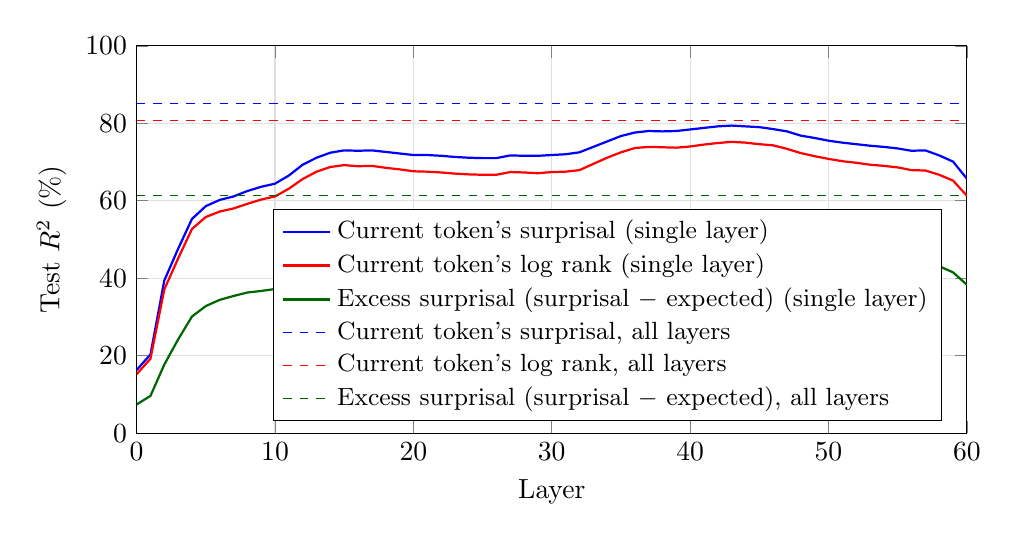
\begin{tikzpicture}
    \begin{axis}[
        width=\linewidth, height=6.5cm,
        xlabel={Layer}, ylabel={Test $R^2$ (\%)},
        xmin=0, xmax=60, ymin=0, ymax=100,
        xtick={0,10,20,30,40,50,60},
        grid=major, grid style={gray!25},
        legend pos=south east, legend cell align=left,
        legend style={font=\small},
      ]
      \addplot[thick, blue, mark=none] coordinates {
        (0,16.3) (1,20.3) (2,39.4) (3,47.6) (4,55.3) (5,58.6) (6,60.2) (7,61.1) (8,62.5) (9,63.6)
        (10,64.4) (11,66.5) (12,69.3) (13,71.1) (14,72.4) (15,73.0) (16,72.9) (17,73.0) (18,72.6) (19,72.2)
        (20,71.8) (21,71.8) (22,71.6) (23,71.3) (24,71.1) (25,71.0) (26,71.0) (27,71.7) (28,71.6) (29,71.6)
        (30,71.8) (31,72.0) (32,72.5) (33,73.9) (34,75.3) (35,76.7) (36,77.6) (37,78.0) (38,77.9) (39,78.0)
        (40,78.4) (41,78.8) (42,79.2) (43,79.4) (44,79.2) (45,79.0) (46,78.5) (47,77.9) (48,76.8) (49,76.2)
        (50,75.5) (51,75.0) (52,74.6) (53,74.2) (54,73.9) (55,73.5) (56,72.9) (57,73.0) (58,71.7) (59,70.1)
        (60,65.7)
      };
      \addlegendentry{Current token's surprisal (single layer)}
      \addplot[thick, red, mark=none] coordinates {
        (0,15.2) (1,19.2) (2,37.1) (3,45.1) (4,52.7) (5,55.8) (6,57.2) (7,58.0) (8,59.2) (9,60.3)
        (10,61.1) (11,63.1) (12,65.6) (13,67.5) (14,68.7) (15,69.2) (16,68.9) (17,69.0) (18,68.5) (19,68.1)
        (20,67.6) (21,67.5) (22,67.3) (23,67.0) (24,66.8) (25,66.7) (26,66.7) (27,67.4) (28,67.3) (29,67.1)
        (30,67.4) (31,67.5) (32,67.9) (33,69.5) (34,71.1) (35,72.5) (36,73.6) (37,73.9) (38,73.8) (39,73.7)
        (40,74.0) (41,74.5) (42,74.9) (43,75.2) (44,75.0) (45,74.6) (46,74.3) (47,73.4) (48,72.3) (49,71.5)
        (50,70.8) (51,70.2) (52,69.8) (53,69.3) (54,69.0) (55,68.6) (56,67.9) (57,67.8) (58,66.7) (59,65.2)
        (60,61.3)
      };
      \addlegendentry{Current token's log rank (single layer)}
      \addplot[thick, black!60!green, mark=none] coordinates {
        (0,7.4) (1,9.6) (2,17.7) (3,24.2) (4,30.1) (5,32.8) (6,34.4) (7,35.4) (8,36.3) (9,36.7)
        (10,37.2) (11,38.8) (12,42.4) (13,44.6) (14,45.9) (15,47.3) (16,46.9) (17,46.5) (18,45.5) (19,44.9)
        (20,44.1) (21,44.2) (22,43.7) (23,43.4) (24,43.1) (25,42.5) (26,42.2) (27,42.9) (28,42.8) (29,42.7)
        (30,43.0) (31,43.4) (32,43.6) (33,45.6) (34,47.4) (35,49.7) (36,50.8) (37,51.8) (38,51.4) (39,51.5)
        (40,52.1) (41,52.5) (42,53.6) (43,54.5) (44,53.6) (45,53.0) (46,52.1) (47,51.6) (48,50.0) (49,48.5)
        (50,47.5) (51,46.6) (52,46.0) (53,45.4) (54,44.9) (55,44.2) (56,43.7) (57,45.0) (58,43.1) (59,41.5)
        (60,38.3)
      };
      \addlegendentry{Excess surprisal (surprisal $-$ expected) (single layer)}
      \addplot[blue, dashed] coordinates {(0,85.0) (60,85.0)};
      \addlegendentry{Current token's surprisal, all layers}
      \addplot[red, dashed] coordinates {(0,80.8) (60,80.8)};
      \addlegendentry{Current token's log rank, all layers}
      \addplot[black!60!green, dashed] coordinates {(0,61.4) (60,61.4)};
      \addlegendentry{Excess surprisal (surprisal $-$ expected), all layers}
    \end{axis}
  \end{tikzpicture}
  \caption{Test $R^2$ for decoding text statistics from a linear probe on one layer's activations at the current token. Dashed: one probe on all 61 layers. Single-layer peaks: current token's surprisal layer 43, current token's log rank layer 43, excess surprisal (surprisal $-$ expected) layer 43.}
  \label{fig:layer-r2-decoded-b}
\end{figure}
